\documentclass{overturerep}

\usepackage{graphics}
\usepackage{times}
\usepackage{listings}
%\usepackage{color}
\usepackage[usenames,dvipsnames]{color}
\usepackage{graphicx}
\usepackage{latexsym}
\usepackage{longtable} % ,multirow}
\usepackage{hyperref}
\usepackage{float}


\floatstyle{ruled}
\newfloat{program}{thp}{lop}
\floatname{program}{Extension point}

\newcommand{\vdmtools}{VDMTools}
\newcommand{\vdmstyle}[1]{\texttt{#1}}
\newcounter{exerciseno}

%\newcommand{\Exercise}[1]{%
%    \textbf{Exercise \thechapter.\theexerciseno}
%   \refstepcounter{exerciseno} #1 $\Box$\\ }%}
%\newcommand{\initexercise}{\setcounter{exerciseno}{0}}
%\newcounter{exerciseno}

\newcommand\thebookexercise{\thechapter.\arabic{exerciseno}}
\newenvironment{myexercise}{\par
  \refstepcounter{exerciseno}%
  \indent\textbf{Exercise\ \thebookexercise}\enskip}{$\Box$\\
}
\newenvironment{myhardexercise}{\par
  \refstepcounter{exerciseno}%
  \indent\textbf{Exercise\ \thebookexercise $\star$}\enskip}{$\Box$\\
}
\newcommand{\initexercise}{\setcounter{exerciseno}{0}}
\newenvironment{mysolution}{
} %% This will be replaced by a perl script extracting the solutions
  %% and inserting them automatically into the solutions chapter.
 

%\newcommand{\insertcommentedvdm*}[2]{}
  %% This macro is identified by perl script which will move the
  %% parameter to the solutions chapter.
% definition of VDM++, JavaCC, JJTree, JTB, ANTLR and SableCC for listings
\lstdefinelanguage{VDM++}
  {morekeywords={act, active, fin, req, waiting, abs, all, allsuper, always, and, answer, 
     assumption, async, atomic, be, bool, by, card, cases, char, class, comp, compose, conc, cycles,
     dcl, def, definitions, del, dinter, div, dlmodule, do, dom, dunion, duration, effect, elems, else, elseif, end,
     error, errs, exists, exists1, exit, exports, ext, floor, for, forall, from, functions, 
     general, hd, if, imports, in, inds, infer, init, inmap, input, instance, int, inter, inv, inverse, iota, is, 
     isofbaseclass, isofclass, inv, inverse, lambda, len, let, map, measure, mu,
     mutex, mod, module, nat, nat1, new, merge, 
     munion, not, of, operations, or, others, per, periodic, post, power, pre, pref, 
     private, protected, public, qsync, rd, responsibility, return, reverse,  
     sameclass, parameters, psubset, rem, renamed, rng, sel, self, seq, seq1, set, skip, specified, st, 
     start, startlist, state, static, subclass, subset, subtrace, sync, system, then, thread, 
     threadid, time, tixe, tl, to, token, traces, trap, types, undefined,
     union, uselib, using, values, 
     variables, while, with, wr, yet, RESULT, false, true, nil, periodic pref, rat, real},
   %keywordsprefix=mk\_,
   %keywordsprefix=a\_,
   %keywordsprefix=t\_,
   %keywordsprefix=w\_,
   sensitive,
   morecomment=[l]--,
   morestring=[b]",
   morestring=[b]',
  }[keywords,comments,strings]
\lstdefinelanguage{JavaCC}
  {morekeywords={options, PARSER\_BEGIN, PARSER\_END, SKIP, TOKEN},
   sensitive=false,
  }[keywords]

% define the layout for listings
\lstdefinestyle{tool}{basicstyle=\ttfamily,
                         frame=trBL, 
			 showstringspaces=false, 
			 frameround=ffff, 
			 framexleftmargin=0mm, 
			 framexrightmargin=0mm}
\lstdefinestyle{mystyle}{basicstyle=\ttfamily,
                         frame=trBL, 
%                         numbers=left, 
%			 gobble=0, 
			 showstringspaces=false, 
%			 linewidth=\textwidth, 
			 frameround=fttt, 
			 aboveskip=5mm,
			 belowskip=5mm,
			 framexleftmargin=0mm, 
			 framexrightmargin=0mm}




%\lstdefinestyle{mystyle}{basicstyle=\sffamily\small,
%			 frame=tb,
%                         numbers=left,
%			 gobble=0,
%			 showstringspaces=false,
%			 linewidth=345pt,
%			 frameround=ffff,
%			 framexleftmargin=8mm,
%			 framexrightmargin=8mm,
%			 framextopmargin=1mm,
%			 framexbottommargin=1mm,
%			 aboveskip=7mm,
%			 belowskip=5mm,
%			 xleftmargin=10mm,}

\lstset{style=mystyle}
\lstset{language=VDM++}
\lstset{alsolanguage=Java}
% The command below enables you to escape into normal LaTeX mode inside your 
% VDM chunks by starting with a `?� character and ending with a `��
%\lstset{escapeinside=?�}

\newcommand{\kw}[1]{{\tt #1}}

%%%%%%%%%%%%%%%%%% Commands for bibtex %%%%%%%%%%%%%%%%%%%%%%%
%************************************************************************
%                                                                       *
%       Bibliography and Terminology supporting commands                *
%                                                                       *
%************************************************************************

\newcommand{\bthisbibliography}[1]{\chapter*{References}%
   \begin {list} {}%
     {\settowidth {\labelwidth} {[#1]XX}%
      \setlength {\leftmargin} {\labelwidth}%
      \addtolength{\leftmargin} {\labelsep}%
      \setlength {\parsep} {1ex}%
      \setlength {\itemsep} {2ex}%
     }
  }
\newcommand{\ethisbibliography}{\end{list}}
\newcommand{\refitem}[2]
  {\bibitem[#1]{#2}}

% Requirements environment
\newenvironment{reqs}{%
\begin{enumerate}
%\renewcommand{\labelenumi}{\textbf{R\theenumi}}
\renewcommand{\theenumi}{\textbf{R\arabic{enumi}}}
}{%
\end{enumerate}}

%\newcommand{\Exercise}[1]{%
%    \textbf{Exercise \thechapter.\theexerciseno}
%   \refstepcounter{exerciseno} #1 $\Box$\\ }%}
%\newcommand{\initexercise}{\setcounter{exerciseno}{0}}

\newcommand{\experience}[1]{%
\begin{center}
\fbox{
\begin{minipage}[t]{.8\textwidth}
#1
\end{minipage}}
\end{center}}

\newcommand{\markDone}[1]{{\color{Gray}#1}}
\newcommand{\developer}[1]{{\scriptsize \fbox{#1}}}


\usepackage{fancyhdr}

\pagestyle{fancy}
\fancyhead{}
\fancyhead[LO]{\leftmark}
\fancyhead[RE]{Necessary adjustments of the Overture/VDM interpreter}
\fancyhead[RO,LE]{\resizebox{0.05\textwidth}{!}{
\includegraphics{OMLlogoattempt.jpg}}}
\fancyfoot[C]{\thepage}


%%%%%%%%%%%%%%%%%%%%%% Commands associated with development docs
\newcommand{\epoint}[1]{{\tt #1}}
\newcommand{\class}[1]{\textit{#1}}
\newcommand{\java}[1]{{\tt #1}}
\newcommand{\lstjava}[1]{
	\lstset
	{
		language=Java,
		basicstyle=\ttfamily\footnotesize,
		captionpos=b,
		caption=#1
	}
}



 
\title{Necessary adjustments of the Overture/VDM interpreter}
\author{P.G. Larsen, IHA \\
   S. Wolff, Terma/IHA \\
   K. Lausdahl, IHA \\
   M. Verhoef, Chess\\
   N. Battle, Fujutsu Services
}

\date{February 2010}

\begin{document}

%\frontmatter
\reportno{TR-2010-05}     

\pagenumbering{roman}
\maketitle
%\addtocounter{page}{2}
\tableofcontents
\newpage

\section*{Document History}
\begin{center}
\begin{tabular}{|c|c|c|}
\hline
\textbf{Revision} & \textbf{Notes} & \textbf{Date} \\ \hline
0.1 & Initial version & 02.2010 \\ \hline
\end{tabular}
\end{center}

\newpage

\pagenumbering{arabic} 
\setcounter{page}{1}

\section{Introduction}

This small memo aims to provide an overview of the adjustments to the
Overture/VDM interpreter in order for the multi-threaded and
multi-processor interpretation to work appropriately and subsequently
pave the way for the co-simulation with 20-sim in the DESTECS project.

\section{Main issues that needs addressing}

The current version of the Overture/VDM interpreter have a number of
issues which definitely needs to be addressed to make it useful for modeling
and validation of multi-threaded VDM++ and VDM-RT models. The main
points are:

\begin{enumerate}
\item Whenever a multi-threaded VDM model is present, the interpreter
  make use of multiple Java threads resulting in a
  non-deterministic execution of such models where errors envisaged
  can be hard to reproduce.
\item Whenever the interpretation is stopped with a breakpoint in the
  interpretation of a multi-threaded VDM model only the thread reaching
  the breakpoint is stopped (or threads that are created in a break
  state). This means that other threads continue their execution. This
  is not the way this should work since these other
  threads will be able to advance much longer than envisaged and it is
  impossible to inspect the exact position of the thread execution and
  inspect the value of the instance variables and local variables.
\item The permission predicates are only reevaluated periodically (in
  relation to the real time of an interpretation) and not whenever its
  value have potentially changed due to the dependencies of the
  history counters and the instance variables adjusted. This means
  that windows of opportunities where the permission predicates can
  enable the blocked threads to continue are not exploited.
\item Only explicit duration and cycle statements will move the
  simulated time. This severely hinders the realistic expectations one
  can have to the model execution in relation to an execution of a
  subsequent implementation. Thus, default durations needs to be
  introduced for all parts of the language and these will need to be
  taken into account.
\end{enumerate}

\section{Main issues that would be nice to address}

In addition to the issues that needs to be solved there are a number of
issues which have been discussed at different points of time and are
desirable in the longer term to enable as well. The list of these
issues include:

\begin{enumerate}
\item Handling of static instance variables in instances of classes
  that are deployed to multiple cpus are not done appropriately
  right now (nor in VDMTools). In essence, if such an instance variable
  is updated in one cpu it is instantly also available at the other
  cpus where it is deployed. This is naturally cheating compared to a
  real world. This may require a language change so this needs to be
  clarified and a proposal will have to be made for the LB when this
  is done.
\item At the moment the deployment of instances of classes happen
  statically in the system class constructor (also in VDMTools). When
  one wish to use the VDM-RT dialect to describe a system where the
  different instances actually physically move and change their
  deployment dynamically this is not appropriate. A new MSc student
  will explore whether it is possible to incorporate concepts for
  dynamic allocation (for example inspired from the CREDO project) in
  a VDM-RT context. This again will probably require language changes
  so it needs to be approved by the LB but it would be advantageous to
  be able to conduct the research for such an extension before
  deciding upon whether it shall be permanently incorporated into
  Overture or not.
\item It would be desirable to be able to use duration intervals
  instead of simply a fixed amount, and then be able to run the
  execution in different modes (smallest number, random but controlled
  by seed or largest numbers).
\item At the moment both Overture/VDM and VDMTools have a single
  virtual cpu containing all the environment functionality. It would
  be desirable to explore the possibility of defining multiple virtual
  cpus for the system class.
\item Incorporation of predicates of events happening over time
  (either dynamically or with post-analysis after the execution based
  on a logfile) would be desirable. Whenever such timed predicates are
  broken the user should easily be able to determine the cause of the
  violation (either if stopped immediately when it was broken or
  graphically in visualizations of logfiles). Another option would be to
  incorporate a special keyword: \emph{maxDuration} for use in post 
  conditions, to describe the maximum allowed duration of the given 
  operation.
\end{enumerate}

\section{Suggested Solutions}

It is suggested to keep the use of Java threads in the Overture/VDM
interpreter but have a master thread which controls all threads. This
master will then act as the overall scheduler in case multi-threaded
VDM models are to be interpreted. Thus there will at any point of time
just be one thread executing and thus the nondeterminism arising from
the Java virtual machine will be eliminated. In addition, the problem
about stopping threads at breakpoints will disappear. Concerning the
reevaluation of permission predicates, additions will need to be
inserted in the Overture/VDM interpreter for this. Essentially this
boils down to a static analysis of all the permission predicates where
dependency information is derived at initialisation time. Subsequently,
this information is to be used by the scheduler whenever any of the
things dependent upon for a block permission predicate is updated.

Talking about the VDM-RT interpreter, the master thread will need
to carry out a round-robin investigation of what functionality each
resource (cpu and bus) can execute before updating the time. Once
all have been processed the smallest time step will be
chosen and all threads will be moved forward with this amount of
time. For the treads that have a longer duration this means that the
remaining duration will be decremented accordingly. For threads that
have durations equal to the minimum duration the transactions
performed in that local thread will be committed and made available to
all other threads. This is also the place where the co-simulation
will be incorporated (before the cpus are asked to progress time with
the smallest time step, the continuous-time model will be asked to progress
this amount of time. Either the continuous-time model will increase time 
by the negotiated amount and values will be exchanged between the two
models, or an event happen at an earlier time and then all
cpus are asked to progress by that amount). 

\section{Handling of Breakpoints}

Several minor corrections to the way breakpoints are handled in the debugger is desired. The following definitions will be used:

\begin{itemize}
	\item Resume
	\item Suspend
	\item Terminate
	\item Step Into
	\item Step Over
	\item Step Return
\end{itemize}

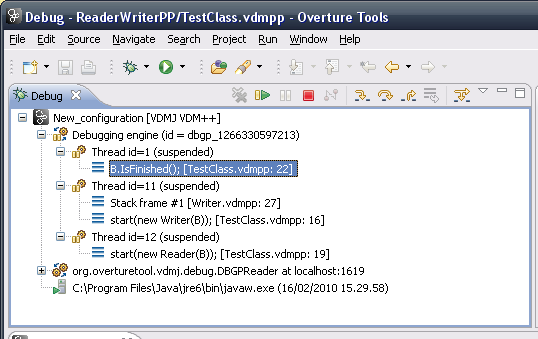
\includegraphics[width=369pt]{figures/stackTrace.png}

When reaching a breakpoint during debugging, the thread reaching the breakpoint should be marked and the source location of the breakpoint should be shown. The following outline would be desirable:

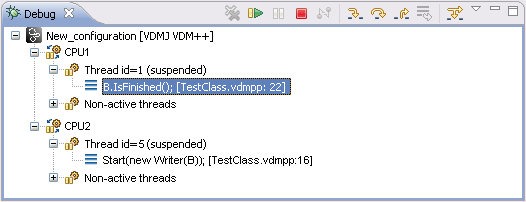
\includegraphics[width=369pt]{figures/NewDebugLook.png}

All cpus are shown on the first level of the debug view. For each cpu, the currently active thread is shown on top, with the option of expanding the list of threads in order to display all threads deployed to the cpu. This will ensure that the active threads are visible at a glance, and give a good overview of the architecture of the system. In addition, all sleeping threads can still be examined should the user wish to. 

\begin{itemize}
	\item When a breakpoint is reached all threads shall stop before the next evaluation.
\end{itemize}

When the user selects:

\begin{itemize}
	\item Terminate: The model is killed. The root process should die.
	\item Resume: The current thread and all other threads are resumed and will only stop again it the Suspend button is pressed or a breakpoint is reached.
	\item Step:
\begin{itemize}
	\item All other threads than the selected one are resumed. The one selected is allowed to evaluate one step of time. Eventually the other threads will stop because of synchronization constraints. New periodic threads must not be allowed to start before the debugging thread has done enough time steps to allow a new scheduling of a new periodic thread.
\end{itemize}

\end{itemize}

\bibliographystyle{newalpha}

\bibliography{bib/bibliography}

\end{document}
